\graphicspath{
    {figures_and_references/evacuation_japan/}
}

% \selectlanguage{english}
\renewcommand{\chapternametext}{Chapter \thechapter . Use case: Evacuation route assessment for Tsunami events in Japan}
\renewcommand{\shortchapternametext}{Chapter \thechapter . Use case: Evacuation route assessment}


\chapter{\chapternametext}
\

\renewcommand{\headingtextL}{}
\renewcommand{\headingtextR}{\shortchapternametext}
\begingroup
 \flushbottom
 \setlength{\parskip}{0pt plus 1fil}%
 \localtableofcontents 
\endgroup

\begingroup
 \flushbottom
 \setlength{\parskip}{0pt plus 1fil}%
 \locallistoffigures
 \locallistoftables
\endgroup


\newpage

\setcounter{section}{0} 

\FloatBarrier

\renewcommand{\sectionnametext}{Introduction}
\renewcommand{\headingtextL}{\shortchapternametext}
\renewcommand{\headingtextR}{\thesection. \sectionnametext}
\section{\sectionnametext}

After assessing seismic hazard and risk, an important next step is evaluating the potential impact of a seismic event on the exposed population and planning effective evacuation strategies. While traditional risk assessments often focus on residential exposure and direct physical damage, emergency management requires a broader perspective that considers how people can safely move through the affected territory during and after a hazardous event. In particular, disruptions to transportation networks, blocked routes, and the accessibility of safe areas can significantly influence the final consequences of a disaster.

One promising approach for addressing this challenge is the evaluation of population accessibility to safe locations. Accessibility-based methodologies consider not only the distance required to reach a safe area but also the quality and effectiveness of the destination itself. Such approaches provide a more realistic representation of evacuation conditions and can support decision-making processes related to emergency planning and risk reduction.

As a preliminary exploration of this research direction, and to illustrate a potential extension of the seismic risk framework developed in this work, a simplified tsunami evacuation accessibility analysis is presented. The case study focuses on a tsunami-prone area in Japan and demonstrates how elevation data, transportation networks, and accessibility metrics can be combined to identify areas with different levels of evacuation safety. This example serves as a proof of concept and highlights future research opportunities aimed at integrating evacuation accessibility analyses with seismic risk and population exposure assessments.
A Python Jupyter notebook demonstrating this use case is available at
\url{https://github.com/CityScope/UrbanAccessAnalyzer} (in the \texttt{examples} folder).

\renewcommand{\sectionnametext}{Methodology and Setup}
\renewcommand{\headingtextR}{\thesection. \sectionnametext}
\section{\sectionnametext}

The objective of this experiment is to develop a data-driven framework for evaluating tsunami evacuation safety within a selected area. The methodology combines topographic information, transportation networks, and accessibility analysis to estimate how easily the population can reach safe locations located above critical elevation thresholds.

Unlike approaches that only identify potentially safe areas, the proposed framework evaluates both the physical protection provided by elevation and the accessibility of those areas through the existing street network. The resulting metric provides a continuous representation of evacuation quality across the study area.

\subsection{Safety Evaluation Criteria}

Tsunami evacuation safety is modelled as the combination of two complementary factors:

\begin{itemize}
    \item \textbf{Elevation Safety}: Higher ground provides greater protection against tsunami inundation. Locations at low elevations receive low safety scores, while locations situated at higher elevations receive progressively higher scores.
    
    
    \item \textbf{Distance to Safety}: The probability of successful evacuation decreases as travel distance increases. Consequently, locations closer to safe areas receive higher accessibility scores. 
\end{itemize}

Both factors are normalized to values between 0 and 1 and combined using a multiplicative formulation:

\begin{equation}
S_{\mathrm{final}} = S_{\mathrm{height}} \times S_{\mathrm{distance}}
\end{equation}

This formulation ensures that a location can only obtain a high safety score when it simultaneously satisfies both criteria. Poor performance in either elevation or accessibility directly reduces the final evacuation quality.

\subsection{Safety Score Definition}

To illustrate the relationship between elevation and evacuation distance, table \ref{tab:tsunami_score} presents an example scoring scheme used to classify tsunami evacuation quality. Higher elevations and shorter evacuation distances result in larger safety scores, while low elevations combined with long travel distances produce lower values.

\begin{table}[htbp]
    \centering
    \caption{Accessibility values as a function of height and walking distance.}
    \label{tab:tsunami_score}

    \setlength{\tabcolsep}{6pt} % improves spacing
    \renewcommand{\arraystretch}{1.2} % improves row height

    \begin{tabular}{c| ccccccccc}
        \hline
        Height (m) & \multicolumn{9}{c}{Walking distance (m)} \\
        \cline{2-10}
        & 50 & 100 & 150 & 200 & 250 & 300 & 350 & 400 & 450 \\
        \hline
        2  & 0   & 0   & 0   & 0   & 0   & 0   & 0   & 0   & 0 \\
        4  & 0.2 & 0.2 & 0.2 & 0.2 & 0.2 & 0.2 & 0.2 & 0.2 & 0 \\
        6  & 0.4 & 0.4 & 0.2 & 0.2 & 0.2 & 0.2 & 0.2 & 0.2 & 0 \\
        8  & 0.4 & 0.4 & 0.4 & 0.4 & 0.2 & 0.2 & 0.2 & 0.2 & 0 \\
        10 & 0.6 & 0.6 & 0.4 & 0.4 & 0.4 & 0.2 & 0.2 & 0.2 & 0 \\
        12 & 0.8 & 0.6 & 0.6 & 0.4 & 0.4 & 0.4 & 0.2 & 0.2 & 0 \\
        14 & 0.8 & 0.8 & 0.6 & 0.6 & 0.4 & 0.4 & 0.2 & 0.2 & 0 \\
        16 & 1.0 & 0.8 & 0.8 & 0.6 & 0.6 & 0.4 & 0.4 & 0.2 & 0 \\
        18 & 1.0 & 1.0 & 0.8 & 0.8 & 0.6 & 0.4 & 0.4 & 0.2 & 0 \\
        \hline
    \end{tabular}
\end{table}

As shown in table \ref{tab:tsunami_score}, the methodology rewards locations that are located at higher elevations and situated closer to safe evacuation zones.

\subsection{Discretization}

To enable efficient computation and spatial analysis, continuous safety values are discretized into a finite number of accessibility levels. Safety scores range from $0$ (completely unsafe) to $1$ (maximum safety). Adaptive discretization schemes are employed to ensure smooth transitions between neighbouring safety classes.

\subsection{Data Sources}

The analysis integrates several geospatial datasets:

\begin{itemize}
\item \textbf{Digital Elevation Model (DEM)}
\begin{itemize}
\item Source: OpenTopography (e.g., COP30).
\item Provides terrain elevation above sea level.
\end{itemize}


\item \textbf{Street Network}
\begin{itemize}
    \item Source: OpenStreetMap.
    \item Processed into a routable graph for accessibility calculations.
\end{itemize}

\item \textbf{Safe Areas}
\begin{itemize}
    \item Generated from elevation contours exceeding selected safety thresholds.
\end{itemize}

\item \textbf{Population Data}
\begin{itemize}
    \item Used to estimate the number of people exposed to different evacuation conditions.
\end{itemize}


\end{itemize}

\subsection{Workflow}

The analysis follows the workflow summarized below:

\begin{enumerate}
\item Define the Area of Interest (AoI).
\item Download and process elevation data.
\item Generate safe areas from elevation thresholds.
\item Build and simplify the street network.
\item Identify safe access points where streets connect to safe areas.
\item Compute network-based accessibility and evacuation distances.
\item Calculate tsunami evacuation safety scores.
\item Integrate population data and derive exposure statistics.
\end{enumerate}

The final output consists of spatially continuous maps representing evacuation quality and population accessibility to safe locations.

\renewcommand{\sectionnametext}{Results}
\renewcommand{\headingtextR}{\thesection. \sectionnametext}
\section{\sectionnametext}

The methodology was applied to the town of Onagawa, Japan, as a demonstration case study.

\begin{figure}[htbp]
\centering
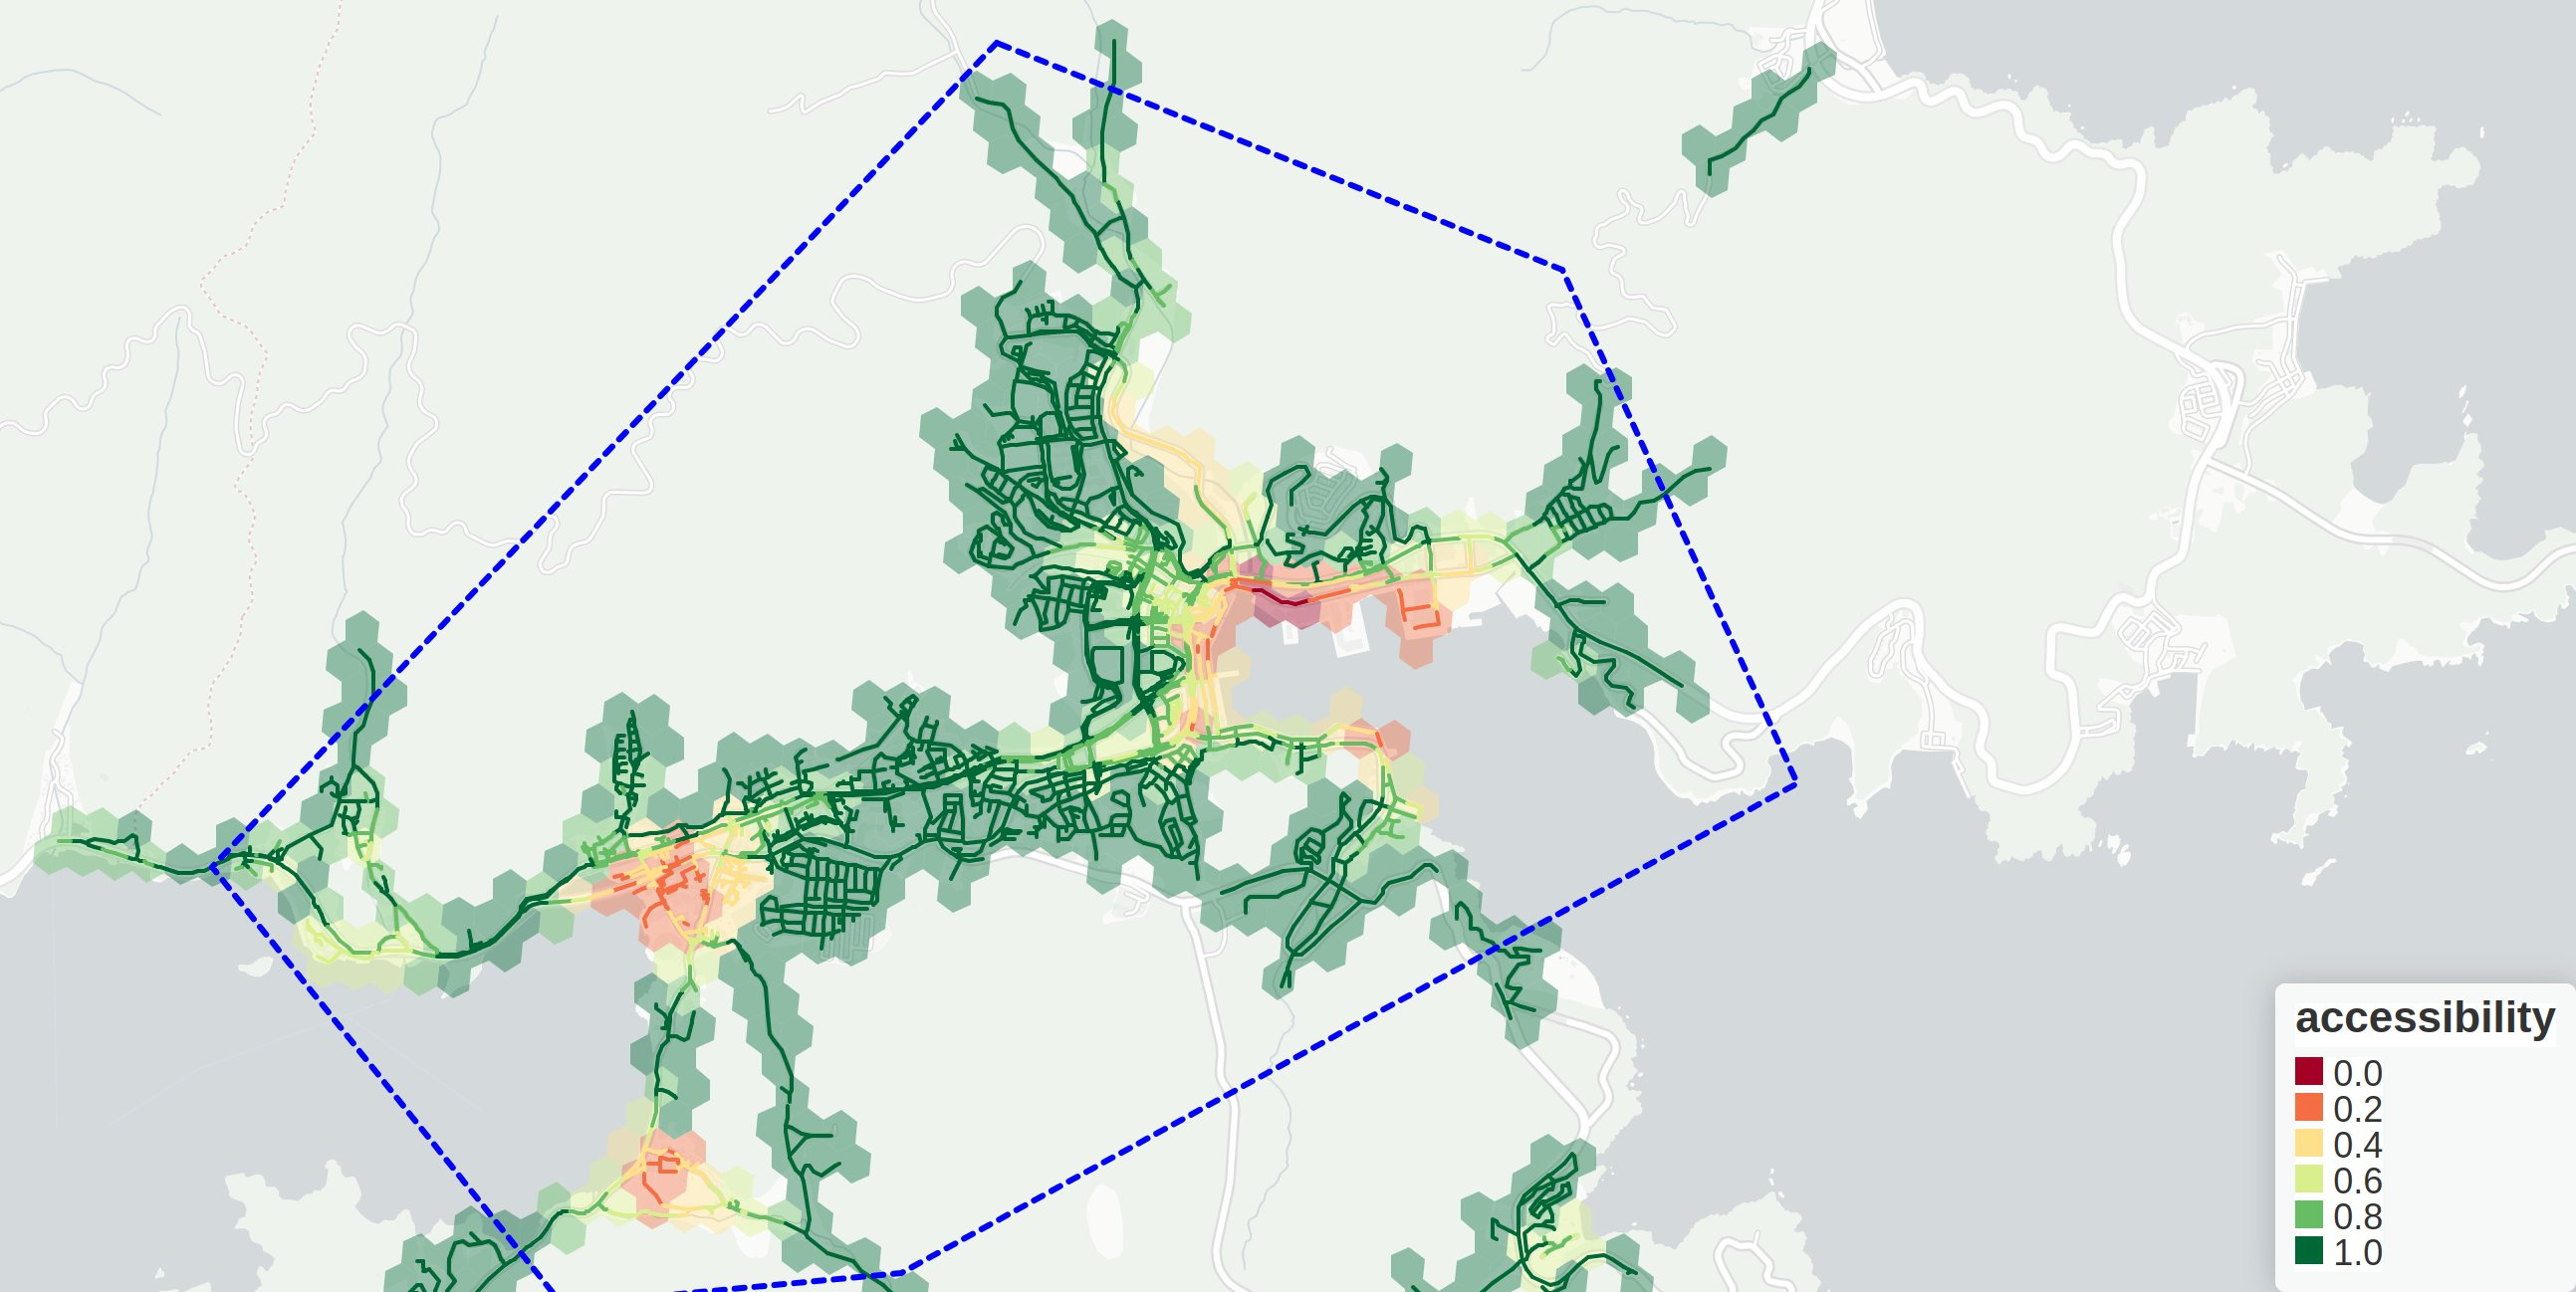
\includegraphics[width=\textwidth]{figures/tsunami_score.jpg}
\caption{Tsunami evacuation score in Onagawa, Japan.}
\label{fig:tsunami_evacuation}
\end{figure}

\begin{figure}[htbp]
\centering
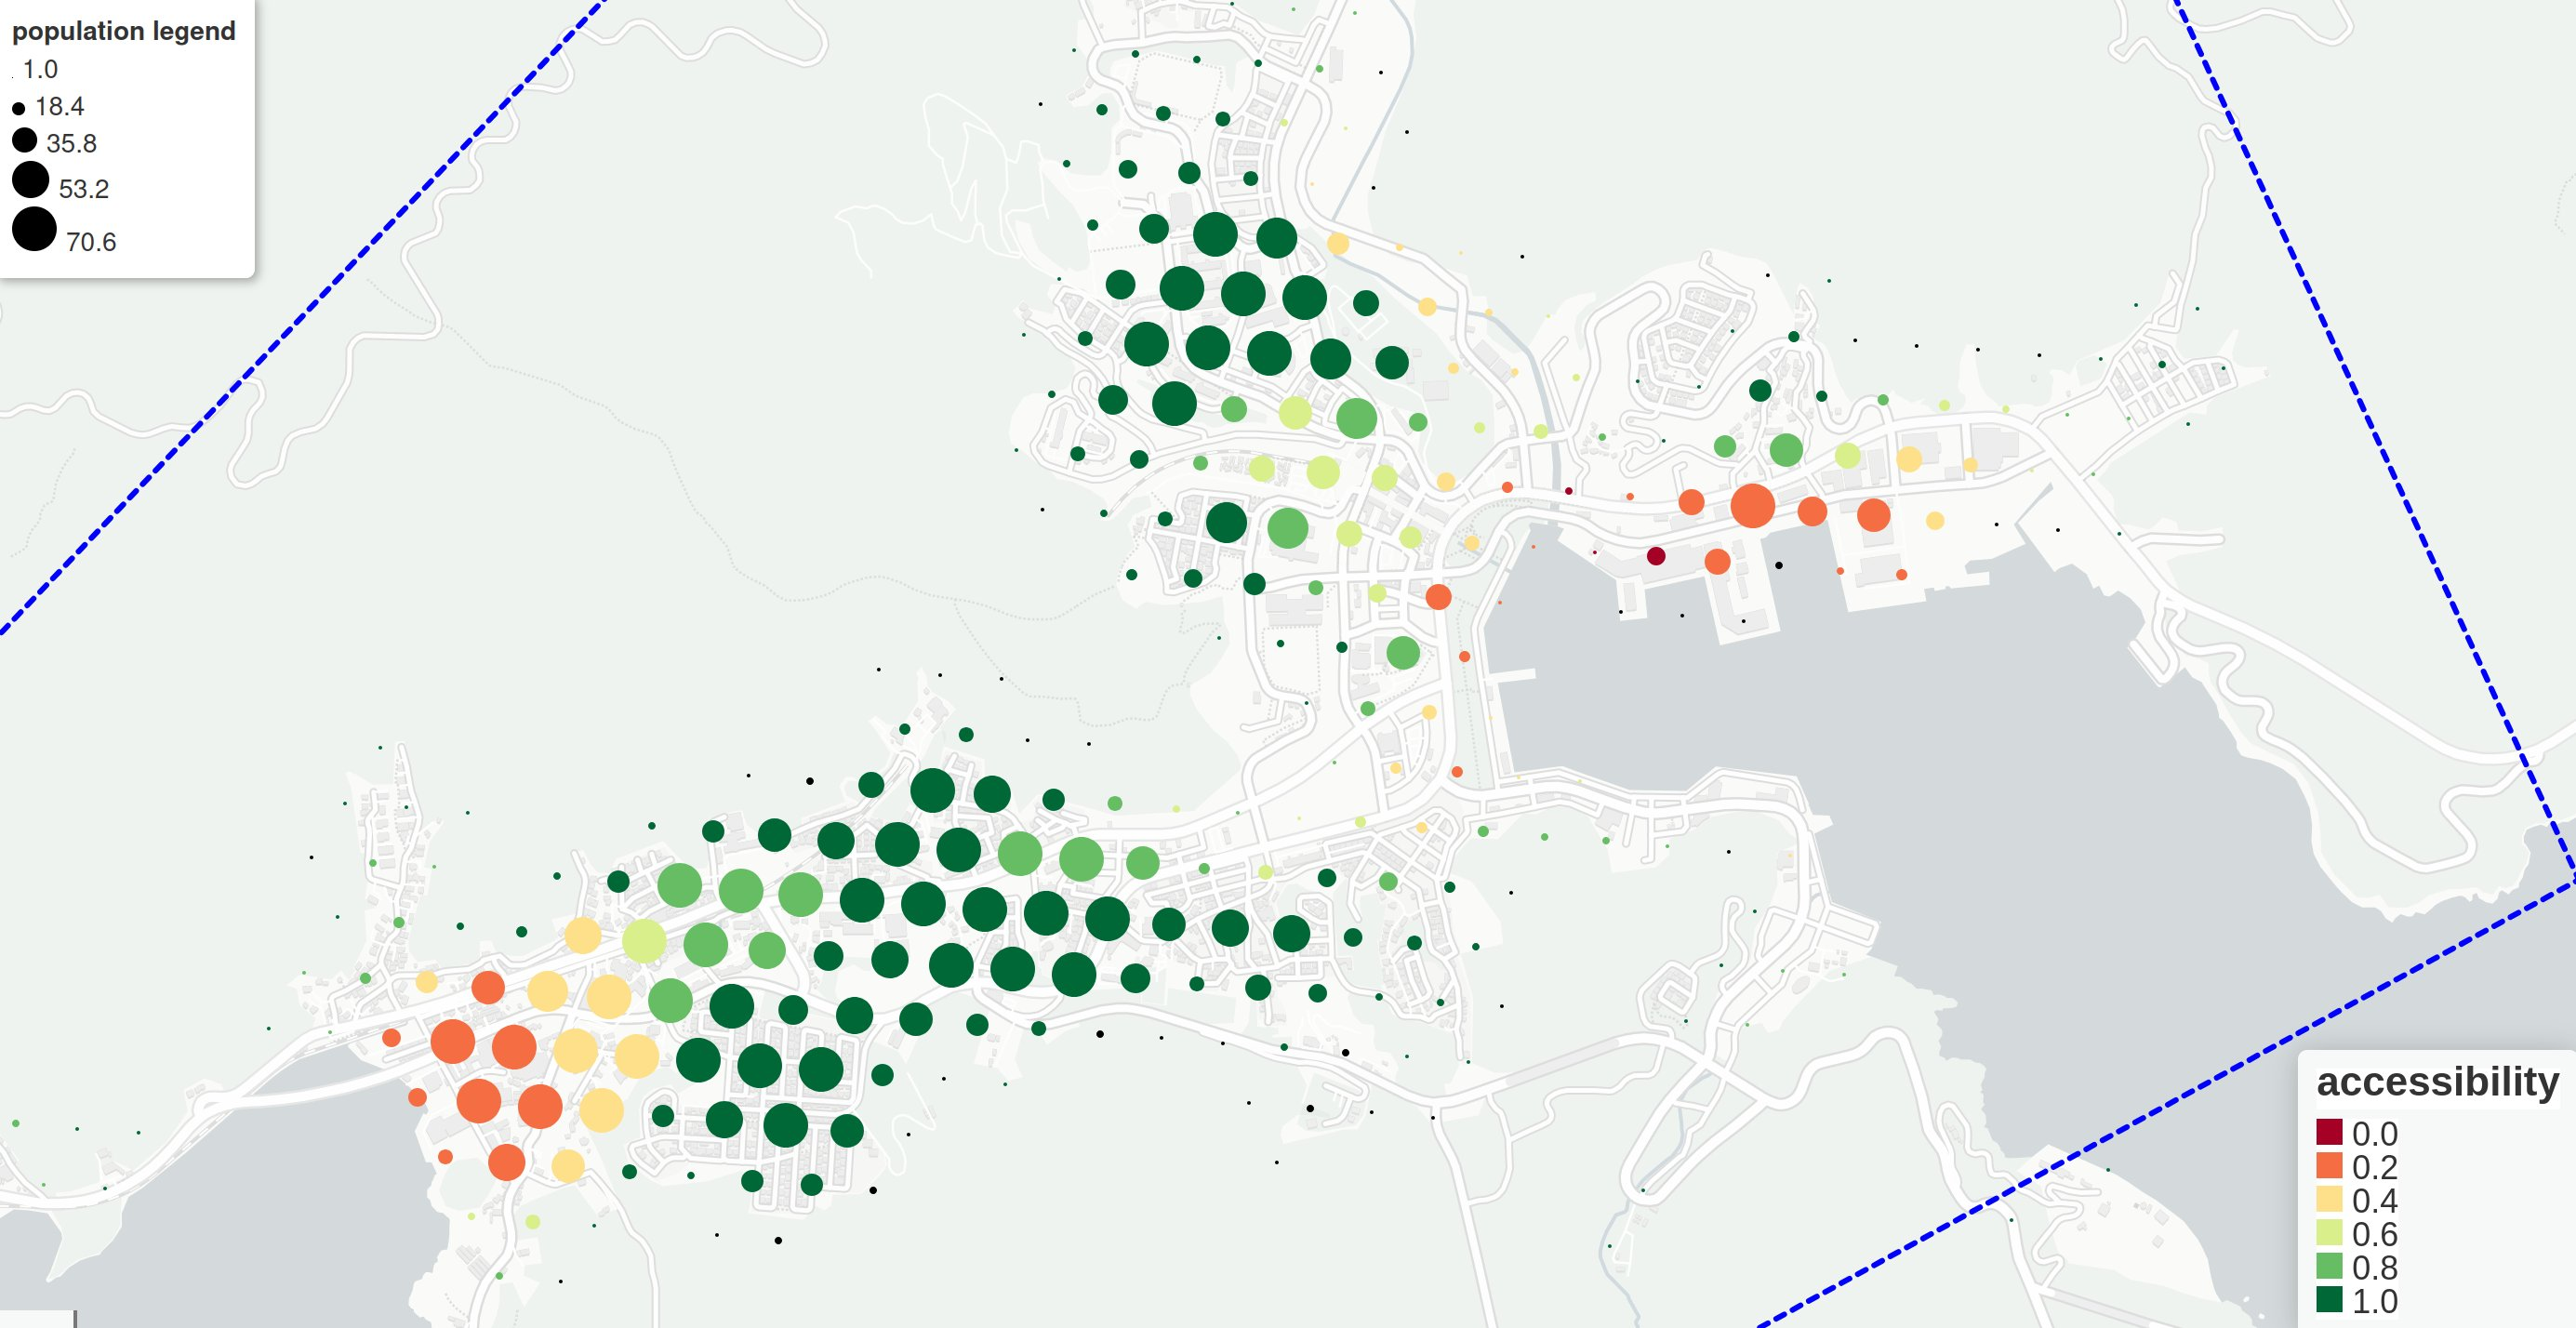
\includegraphics[width=\textwidth]{figures/tsunami_population.jpg}
\caption{Population distribution and tsunami evacuation score in Onagawa, Japan.}
\label{fig:tsunami_pop}
\end{figure}

\begin{table}[h]
\centering
\begin{tabular}{lrr}
\hline
Accessibility & Population & Population (\%) \\
\hline
1.0 & 2249 & 54.18 \\
0.8 & 712 & 17.16 \\
0.6 & 324 & 7.81 \\
0.4 & 445 & 10.72 \\
0.2 & 401 & 9.66 \\
0.0 & 19 & 0.47 \\
Total population & 4152 & 100.00 \\
\hline
\end{tabular}
\caption{Population distribution by safety score level in Onagawa, Japan.}
\label{tab:accessibility_population}
\end{table}

As shown in figures \ref{fig:tsunami_evacuation}, \ref{fig:tsunami_pop} and table \ref{tab:accessibility_population}, the proposed methodology provides a simple and effective way of identifying areas with different levels of evacuation safety. The resulting maps clearly highlight locations where accessibility to safe areas is limited and where the population may face greater challenges during an emergency evacuation.

Although this experiment represents a simplified application focused on tsunami evacuation, it demonstrates the potential of accessibility-based approaches for disaster risk assessment. Future work will focus on integrating this methodology with the broader seismic risk framework developed in this study, allowing the generation of combined risk and population exposure maps that account not only for hazard intensity and building vulnerability but also for evacuation accessibility and emergency response capabilities.
